\section{Discussion}
To understand how open and reproducible data science operates ``under the hood" through critical triggering dynamics, we have measured the response activity following the impulse of the Astro Hack Week , a one week hackathon for astronomers. Our results help describe the complex dynamics, behaviors and tradeoffs faced by the actors of this community, which deserve bringing a broader context. They also open new questions for future research directions.

Our approach, which combines in-depth modeling of actions taken by participants and their dynamics, before, during and after the AstroWeek, with a typical qualitative gathering of ethnographic evidence, brings a broad context view of the long-memory dynamics observed. We have characterized a {\it kairos} moment \cite{orlikowski2002s} of open and reproducible science, focused on community joining and integration, with non trivial spillovers and long-term effects. Nevertheless, our observations suggest that the initial shock, namely, the first day of the AstroWeek, or at least the AstroWeek itself, gives the impulse. Therefore, at least in theory, the larger the initial impulse the more important the long-term response. There are two ways to enhance this peak activity: Either increase the number of participants, or find ways to increase activity with the same number of participants. In practice, tuning the impulse as a parameter, may be more tricky: More participants increase coordination costs, and it is unclear how to boost activity. The impulse may also be conditioned to previous exposure to  collaboration and social interactions.

Similarly, although the exponent $\alpha$, representing the long-memory response (the lower $\alpha$, the slower the decay) seems to be stable and robust across activity types, it remains unclear whether we observed a genuine feature of the AstroWeek, of a more general law of open and reproducible science, or a universal law of open collaboration. The origin of the small exponent ($\alpha \approx 0.25$) requires more investigation. It may stem from the combined effects of cascades of repository creations and critical triggering of contributions. It may also result from complex networks of influence between community members, and even types of events \cite{saichev2013hierarchy}. There is little doubt that the nature of events play a role in the cascading dynamics, yet it remains hard to investigate in detail. In addition, there are multitudes of {\it weak} signal, which cannot be captured either because they are systematically not recorded (e.g. talking at a pub, as shown on Figure \ref{fig:pub}), but also from the GitHub data, which might be too entangled or not significant enough to draw solid conclusions.

\begin{figure}[!t]
\centering
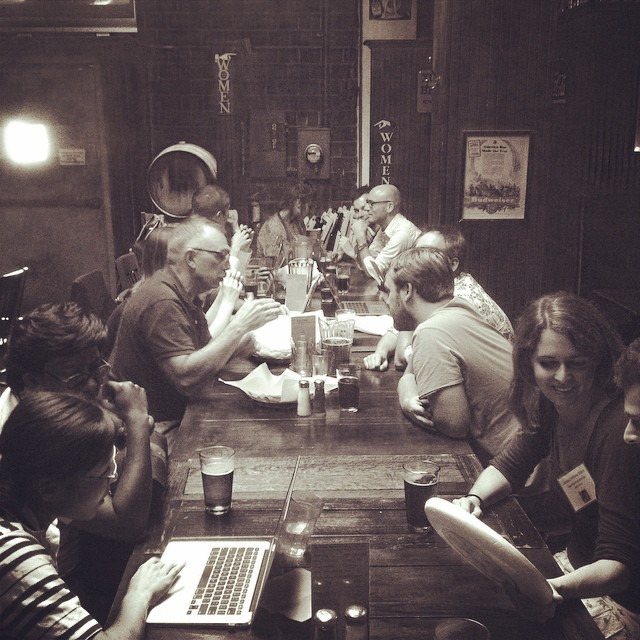
\includegraphics[width=0.9\columnwidth]{figures/pub.jpg}
\caption{Happy hours at Astro Hack Week 2014. Photo by Adrian Price-Whelan. (source: \url{http://astrohackweek.github.io/blog/astro-hack-week-wrapup.html})}
\label{fig:pub}
\end{figure}

This is precisely where the ethnography approach plays a fundamental role to provide context, not only for the dynamics observed and modeled, but also to guide the expert in quantitative social dynamics, in order to ask the good questions and search meaningful information, which might be buried in the ocean of data. For instance, an interviewed senior data scientist (P4), reported that while it was an investment for him to teach at the Astro Hack Week, this event allowed him build social ties with another senior scientist. These social ties have turned into a research project (posted as a repository on GitHub), several months later. In principle, this information could be dug out of the data, but it is less sure whether it would be worth launching a quantitative analysis on these kinds of very long-term follow-up events, without enough contextual information. Having this information in hand, new research paths on the very long-term effects of a hackathon may be quantitatively investigated in the future.

Conversely, the quantitative approach was useful for fact checking of some biased perceptions by interviewees. For instance, a participant believed that activity followed a step function, i.e. little activity before, a lot during, and again little activity after the Astro Hack Week. He was not conscious that follow-up activity really existed in the way we have described.

More broadly, each hackathon is a unique experience bringing its own kind of people. It remains to be seen how the results presented here generalize, and on the contrary, how they constitute the footprint of the Astro Hack Week. Similarly, a larger sample of investigated hackathons would help better identify the rules commons of all hackathons, and at the same time, their unique specificities.

Although GitHub, as well as other social coding platforms, has proven to be very efficient platforms for open and reproducible science collaboration, efforts have been undertaken for a better integration of tools for computational science. For instance, the IPython Notebook has been credited to be ``great for working through things interactively, virtually all [my] work starts here.� Very recently, GitHub has integrated the IPython Notebook viewer (i.e., NB viewer) in its interface, in order to visually render all notebooks stored in GitHub \cite{notebook_rendering}. This example opens the question of the importance of tools in the open and reproducible science process, and how their evolution may additionally change the practice of science. As the practice of science change on open collaboration platform, we shall also witness the evolution of activity patterns, when considering the underlying software used by scientists. Further investigation is necessary to delineate how these increasingly online and web based tools will actually impact the science practice, and whether it is possible to anticipate the evolution of these tools.


%For example, a pattern recognition tool for search and identification of stars, developed by astronomers, may be repurposed for mapping aerial satellite images \cite{kapadia} {\bf [not sure if this example is best]}.

%- find long-term traces of activity (common projects may be initiated months after initial physical meeting $\rightarrow$ kyle interview saying that he has started something with Phill Marshall). Resonates with the very slow (theoretical) decay.


%It's unclear how the social ties established on the long term, triggering collaboration between a subset of the community several months or even years after the Astro Hack Week, may be traced back through the empirical dynamics, to the original encounter. However, the structure interview may greatly help bridge this gap. For instance, when asked about long-term spillovers and benefits of the Astro Hack Week, a senior participant indicated that he started a research project in collaboration with two other senior data scientists, whom he had met and got to know during the Astro Hack Week. Such indication, may help trace meaningful ties between events, which otherwise would be buried into the ambient activity, and for which getting statistical significance of causality, may simply be impossible.


%one point statistics: we shall see it what fashion it will repeat in Astro Hack Week 2015, or in similar events. We shall not presume that all events have the same response dynamics (we have preliminary evidence that another event, involving the astro community has happened earlier in 2014, with slightly different dynamics). We shall on the contrary leverage our proposed method combining quantitive modeling with structured interviews, to bring deep insights, on the complex dynamics and social interactions, occurring during data science events.
